% !TeX encoding = UTF-8
% !TeX spellcheck = en_US

%% bare_conf.tex
%% V1.3
%% 2007/01/11
%% by Michael Shell
%% See:
%% http://www.michaelshell.org/
%% for current contact information.
%%
%% This is a skeleton file demonstrating the use of IEEEtran.cls
%% (requires IEEEtran.cls version 1.7 or later) with an IEEE conference paper.
%%
%% Support sites:
%% http://www.michaelshell.org/tex/ieeetran/
%% http://www.ctan.org/tex-archive/macros/latex/contrib/IEEEtran/
%% and
%% http://www.ieee.org/

%%*************************************************************************
%% Legal Notice:
%% This code is offered as-is without any warranty either expressed or
%% implied; without even the implied warranty of MERCHANTABILITY or
%% FITNESS FOR A PARTICULAR PURPOSE! 
%% User assumes all risk.
%% In no event shall IEEE or any contributor to this code be liable for
%% any damages or losses, including, but not limited to, incidental,
%% consequential, or any other damages, resulting from the use or misuse
%% of any information contained here.
%%
%% All comments are the opinions of their respective authors and are not
%% necessarily endorsed by the IEEE.
%%
%% This work is distributed under the LaTeX Project Public License (LPPL)
%% ( http://www.latex-project.org/ ) version 1.3, and may be freely used,
%% distributed and modified. A copy of the LPPL, version 1.3, is included
%% in the base LaTeX documentation of all distributions of LaTeX released
%% 2003/12/01 or later.
%% Retain all contribution notices and credits.
%% ** Modified files should be clearly indicated as such, including  **
%% ** renaming them and changing author support contact information. **
%%
%% File list of work: IEEEtran.cls, IEEEtran_HOWTO.pdf, bare_adv.tex,
%%                    bare_conf.tex, bare_jrnl.tex, bare_jrnl_compsoc.tex
%%*************************************************************************

% *** Authors should verify (and, if needed, correct) their LaTeX system  ***
% *** with the testflow diagnostic prior to trusting their LaTeX platform ***
% *** with production work. IEEE's font choices can trigger bugs that do  ***
% *** not appear when using other class files.                            ***
% The testflow support page is at:
% http://www.michaelshell.org/tex/testflow/



% Note that the a4paper option is mainly intended so that authors in
% countries using A4 can easily print to A4 and see how their papers will
% look in print - the typesetting of the document will not typically be
% affected with changes in paper size (but the bottom and side margins will).
% Use the testflow package mentioned above to verify correct handling of
% both paper sizes by the user's LaTeX system.
%
% Also note that the "draftcls" or "draftclsnofoot", not "draft", option
% should be used if it is desired that the figures are to be displayed in
% draft mode.
%
\documentclass[conference,onecolumn]{IEEEtran}
% Add the compsoc option for Computer Society conferences.
%
% If IEEEtran.cls has not been installed into the LaTeX system files,
% manually specify the path to it like:
% \documentclass[conference]{../sty/IEEEtran}


\usepackage{hyperref}
%\usepackage{listings}
\usepackage{listingsutf8}
\usepackage{graphicx}
\usepackage{placeins}
\usepackage{color}

%\usepackage{amssymb}

%\usepackage{wrapfig}
%\usepackage{float}
%\usepackage{picins}

% Some very useful LaTeX packages include:
% (uncomment the ones you want to load)


% *** MISC UTILITY PACKAGES ***
%
%\usepackage{ifpdf}
% Heiko Oberdiek's ifpdf.sty is very useful if you need conditional
% compilation based on whether the output is pdf or dvi.
% usage:
% \ifpdf
%   % pdf code
% \else
%   % dvi code
% \fi
% The latest version of ifpdf.sty can be obtained from:
% http://www.ctan.org/tex-archive/macros/latex/contrib/oberdiek/
% Also, note that IEEEtran.cls V1.7 and later provides a builtin
% \ifCLASSINFOpdf conditional that works the same way.
% When switching from latex to pdflatex and vice-versa, the compiler may
% have to be run twice to clear warning/error messages.






% *** CITATION PACKAGES ***
%
%\usepackage{cite}
% cite.sty was written by Donald Arseneau
% V1.6 and later of IEEEtran pre-defines the format of the cite.sty package
% \cite{} output to follow that of IEEE. Loading the cite package will
% result in citation numbers being automatically sorted and properly
% "compressed/ranged". e.g., [1], [9], [2], [7], [5], [6] without using
% cite.sty will become [1], [2], [5]--[7], [9] using cite.sty. cite.sty's
% \cite will automatically add leading space, if needed. Use cite.sty's
% noadjust option (cite.sty V3.8 and later) if you want to turn this off.
% cite.sty is already installed on most LaTeX systems. Be sure and use
% version 4.0 (2003-05-27) and later if using hyperref.sty. cite.sty does
% not currently provide for hyperlinked citations.
% The latest version can be obtained at:
% http://www.ctan.org/tex-archive/macros/latex/contrib/cite/
% The documentation is contained in the cite.sty file itself.






% *** GRAPHICS RELATED PACKAGES ***
%
\ifCLASSINFOpdf
  % \usepackage[pdftex]{graphicx}
  % declare the path(s) where your graphic files are
  % \graphicspath{{../pdf/}{../jpeg/}}
  % and their extensions so you won't have to specify these with
  % every instance of \includegraphics
  % \DeclareGraphicsExtensions{.pdf,.jpeg,.png}
\else
  % or other class option (dvipsone, dvipdf, if not using dvips). graphicx
  % will default to the driver specified in the system graphics.cfg if no
  % driver is specified.
  % \usepackage[dvips]{graphicx}
  % declare the path(s) where your graphic files are
  % \graphicspath{{../eps/}}
  % and their extensions so you won't have to specify these with
  % every instance of \includegraphics
  % \DeclareGraphicsExtensions{.eps}
\fi
% graphicx was written by David Carlisle and Sebastian Rahtz. It is
% required if you want graphics, photos, etc. graphicx.sty is already
% installed on most LaTeX systems. The latest version and documentation can
% be obtained at: 
% http://www.ctan.org/tex-archive/macros/latex/required/graphics/
% Another good source of documentation is "Using Imported Graphics in
% LaTeX2e" by Keith Reckdahl which can be found as epslatex.ps or
% epslatex.pdf at: http://www.ctan.org/tex-archive/info/
%
% latex, and pdflatex in dvi mode, support graphics in encapsulated
% postscript (.eps) format. pdflatex in pdf mode supports graphics
% in .pdf, .jpeg, .png and .mps (metapost) formats. Users should ensure
% that all non-photo figures use a vector format (.eps, .pdf, .mps) and
% not a bitmapped formats (.jpeg, .png). IEEE frowns on bitmapped formats
% which can result in "jaggedy"/blurry rendering of lines and letters as
% well as large increases in file sizes.
%
% You can find documentation about the pdfTeX application at:
% http://www.tug.org/applications/pdftex





% *** MATH PACKAGES ***
%
%\usepackage[cmex10]{amsmath}
% A popular package from the American Mathematical Society that provides
% many useful and powerful commands for dealing with mathematics. If using
% it, be sure to load this package with the cmex10 option to ensure that
% only type 1 fonts will utilized at all point sizes. Without this option,
% it is possible that some math symbols, particularly those within
% footnotes, will be rendered in bitmap form which will result in a
% document that can not be IEEE Xplore compliant!
%
% Also, note that the amsmath package sets \interdisplaylinepenalty to 10000
% thus preventing page breaks from occurring within multiline equations. Use:
%\interdisplaylinepenalty=2500
% after loading amsmath to restore such page breaks as IEEEtran.cls normally
% does. amsmath.sty is already installed on most LaTeX systems. The latest
% version and documentation can be obtained at:
% http://www.ctan.org/tex-archive/macros/latex/required/amslatex/math/





% *** SPECIALIZED LIST PACKAGES ***
%
%\usepackage{algorithmic}
% algorithmic.sty was written by Peter Williams and Rogerio Brito.
% This package provides an algorithmic environment fo describing algorithms.
% You can use the algorithmic environment in-text or within a figure
% environment to provide for a floating algorithm. Do NOT use the algorithm
% floating environment provided by algorithm.sty (by the same authors) or
% algorithm2e.sty (by Christophe Fiorio) as IEEE does not use dedicated
% algorithm float types and packages that provide these will not provide
% correct IEEE style captions. The latest version and documentation of
% algorithmic.sty can be obtained at:
% http://www.ctan.org/tex-archive/macros/latex/contrib/algorithms/
% There is also a support site at:
% http://algorithms.berlios.de/index.html
% Also of interest may be the (relatively newer and more customizable)
% algorithmicx.sty package by Szasz Janos:
% http://www.ctan.org/tex-archive/macros/latex/contrib/algorithmicx/




% *** ALIGNMENT PACKAGES ***
%
\usepackage{array}
% Frank Mittelbach's and David Carlisle's array.sty patches and improves
% the standard LaTeX2e array and tabular environments to provide better
% appearance and additional user controls. As the default LaTeX2e table
% generation code is lacking to the point of almost being broken with
% respect to the quality of the end results, all users are strongly
% advised to use an enhanced (at the very least that provided by array.sty)
% set of table tools. array.sty is already installed on most systems. The
% latest version and documentation can be obtained at:
% http://www.ctan.org/tex-archive/macros/latex/required/tools/


%\usepackage{mdwmath}
%\usepackage{mdwtab}
% Also highly recommended is Mark Wooding's extremely powerful MDW tools,
% especially mdwmath.sty and mdwtab.sty which are used to format equations
% and tables, respectively. The MDWtools set is already installed on most
% LaTeX systems. The lastest version and documentation is available at:
% http://www.ctan.org/tex-archive/macros/latex/contrib/mdwtools/


% IEEEtran contains the IEEEeqnarray family of commands that can be used to
% generate multiline equations as well as matrices, tables, etc., of high
% quality.


%\usepackage{eqparbox}
% Also of notable interest is Scott Pakin's eqparbox package for creating
% (automatically sized) equal width boxes - aka "natural width parboxes".
% Available at:
% http://www.ctan.org/tex-archive/macros/latex/contrib/eqparbox/





% *** SUBFIGURE PACKAGES ***
%\usepackage[tight,footnotesize]{subfigure}
% subfigure.sty was written by Steven Douglas Cochran. This package makes it
% easy to put subfigures in your figures. e.g., "Figure 1a and 1b". For IEEE
% work, it is a good idea to load it with the tight package option to reduce
% the amount of white space around the subfigures. subfigure.sty is already
% installed on most LaTeX systems. The latest version and documentation can
% be obtained at:
% http://www.ctan.org/tex-archive/obsolete/macros/latex/contrib/subfigure/
% subfigure.sty has been superceeded by subfig.sty.

%\usepackage[caption=false]{caption}
%\usepackage[font=footnotesize]{subfig}
% subfig.sty, also written by Steven Douglas Cochran, is the modern
% replacement for subfigure.sty. However, subfig.sty requires and
% automatically loads Axel Sommerfeldt's caption.sty which will override
% IEEEtran.cls handling of captions and this will result in nonIEEE style
% figure/table captions. To prevent this problem, be sure and preload
% caption.sty with its "caption=false" package option. This is will preserve
% IEEEtran.cls handing of captions. Version 1.3 (2005/06/28) and later 
% (recommended due to many improvements over 1.2) of subfig.sty supports
% the caption=false option directly:
%\usepackage[caption=false,font=footnotesize]{subfig}
%
% The latest version and documentation can be obtained at:
% http://www.ctan.org/tex-archive/macros/latex/contrib/subfig/
% The latest version and documentation of caption.sty can be obtained at:
% http://www.ctan.org/tex-archive/macros/latex/contrib/caption/




% *** FLOAT PACKAGES ***
%
%\usepackage{fixltx2e}
% fixltx2e, the successor to the earlier fix2col.sty, was written by
% Frank Mittelbach and David Carlisle. This package corrects a few problems
% in the LaTeX2e kernel, the most notable of which is that in current
% LaTeX2e releases, the ordering of single and double column floats is not
% guaranteed to be preserved. Thus, an unpatched LaTeX2e can allow a
% single column figure to be placed prior to an earlier double column
% figure. The latest version and documentation can be found at:
% http://www.ctan.org/tex-archive/macros/latex/base/

%\usepackage{dblfloatfix}

%\usepackage{stfloats}
% stfloats.sty was written by Sigitas Tolusis. This package gives LaTeX2e
% the ability to do double column floats at the bottom of the page as well
% as the top. (e.g., "\begin{figure*}[!b]" is not normally possible in
% LaTeX2e). It also provides a command:
%\fnbelowfloat
% to enable the placement of footnotes below bottom floats (the standard
% LaTeX2e kernel puts them above bottom floats). This is an invasive package
% which rewrites many portions of the LaTeX2e float routines. It may not work
% with other packages that modify the LaTeX2e float routines. The latest
% version and documentation can be obtained at:
% http://www.ctan.org/tex-archive/macros/latex/contrib/sttools/
% Documentation is contained in the stfloats.sty comments as well as in the
% presfull.pdf file. Do not use the stfloats baselinefloat ability as IEEE
% does not allow \baselineskip to stretch. Authors submitting work to the
% IEEE should note that IEEE rarely uses double column equations and
% that authors should try to avoid such use. Do not be tempted to use the
% cuted.sty or midfloat.sty packages (also by Sigitas Tolusis) as IEEE does
% not format its papers in such ways.




% *** PDF, URL AND HYPERLINK PACKAGES ***
%
%\usepackage{url}
% url.sty was written by Donald Arseneau. It provides better support for
% handling and breaking URLs. url.sty is already installed on most LaTeX
% systems. The latest version can be obtained at:
% http://www.ctan.org/tex-archive/macros/latex/contrib/misc/
% Read the url.sty source comments for usage information. Basically,
% \url{my_url_here}.





% *** Do not adjust lengths that control margins, column widths, etc. ***
% *** Do not use packages that alter fonts (such as pslatex).         ***
% There should be no need to do such things with IEEEtran.cls V1.6 and later.
% (Unless specifically asked to do so by the journal or conference you plan
% to submit to, of course. )


% correct bad hyphenation here
\hyphenation{op-tical net-works semi-conduc-tor}

\newcommand{\warning}[1]{{\textcolor{red}{\bf Warning:}}}

\begin{document}
%
% paper title
% can use linebreaks \\ within to get better formatting as desired
\title{ANTLR4EMF\\Project proposal}


% author names and affiliations
% use a multiple column layout for up to three different
% affiliations
\author{\IEEEauthorblockN{Harald A. Weiner}
\IEEEauthorblockA{JKU\\
%Georgia Institute of Technology\\
Linz, Austria\\
Email: harald.weiner@jku.at}}

% conference papers do not typically use \thanks and this command
% is locked out in conference mode. If really needed, such as for
% the acknowledgment of grants, issue a \IEEEoverridecommandlockouts
% after \documentclass

% for over three affiliations, or if they all won't fit within the width
% of the page, use this alternative format:
% 
%\author{\IEEEauthorblockN{Michael Shell\IEEEauthorrefmark{1},
%Homer Simpson\IEEEauthorrefmark{2},
%James Kirk\IEEEauthorrefmark{3}, 
%Montgomery Scott\IEEEauthorrefmark{3} and
%Eldon Tyrell\IEEEauthorrefmark{4}}
%\IEEEauthorblockA{\IEEEauthorrefmark{1}School of Electrical and Computer Engineering\\
%Georgia Institute of Technology,
%Atlanta, Georgia 30332--0250\\ Email: see http://www.michaelshell.org/contact.html}
%\IEEEauthorblockA{\IEEEauthorrefmark{2}Twentieth Century Fox, Springfield, USA\\
%Email: homer@thesimpsons.com}
%\IEEEauthorblockA{\IEEEauthorrefmark{3}Starfleet Academy, San Francisco, California 96678-2391\\
%Telephone: (800) 555--1212, Fax: (888) 555--1212}
%\IEEEauthorblockA{\IEEEauthorrefmark{4}Tyrell Inc., 123 Replicant Street, Los Angeles, California 90210--4321}}




% use for special paper notices
%\IEEEspecialpapernotice{(Invited Paper)}




% make the title area
\maketitle

% !TeX encoding = UTF-8
% !TeX spellcheck = en_US
\begin{abstract}
%\boldmath
This project aims to use a C code parser 
to walk through the produced abstract syntax tree (AST) 
to provide an importer to the {\it ECCO}
({\it Extraction and Composition for Clone-and-Own})
tool. The goal is
to offer case studies for the feature model exploration 
implementations in {\it ECCO}.
Various approaches have been explored and finally
Eclipse MoDisco in combination with the Xtext
plug-in have been chosen to reverse-engineer C programs
and import them into the EMF (Eclipse Modeling Framework).
\end{abstract}


% IEEEtran.cls defaults to using nonbold math in the Abstract.
% This preserves the distinction between vectors and scalars. However,
% if the conference you are submitting to favors bold math in the abstract,
% then you can use LaTeX's standard command \boldmath at the very start
% of the abstract to achieve this. Many IEEE journals/conferences frown on
% math in the abstract anyway.

% no keywords




% For peer review papers, you can put extra information on the cover
% page as needed:
% \ifCLASSOPTIONpeerreview
% \begin{center} \bfseries EDICS Category: 3-BBND \end{center}
% \fi
%
% For peerreview papers, this IEEEtran command inserts a page break and
% creates the second title. It will be ignored for other modes.
\IEEEpeerreviewmaketitle


% % !TeX encoding = UTF-8
% !TeX spellcheck = en_US
\section{Introduction}
\IEEEPARstart{T}his project has been developed as part of my project in software engineering for the master course computer science.
The tool {\it ECCO}
({\it Extraction and Composition for Clone-and-Own})\cite{fischer2014enhancing}
is developed at the ISSE (Institute for Software Systems Engineering \cite{ISSE_URL})
at Johannes Kepler University in Linz, Austria 
and can be found at \cite{ecourl}.
It maps commonalities and differences of existing variants 
of a portfolio to a feature set.
To provide a real-life case study, the Linux Kernel has been chosen as a 
demonstration example for the {\it ECCO} tool 
(the Linux kernel is a pretty well-known example / case study 
and a project with huge impacts in industry and research).
At the moment, plain C and C++ programs are not supported by {\it ECCO} yet.
Therefore, an importer should be written which is
able to use the output of C parsers to extract the relevant information
for {\it ECCO}. 
The  KeFaX project should provide an importer for the Linux kernel to the ECCO tool. 
As a result,
this project is supposed to parse the Linux .config file, 
set-up the minimal infrastructure of source code for the modules and 
parse the source code. At the end, this project should create an ``input tree'' data
structure. 
Various approaches exist which have been evaluated
for their suitability to the given task. 
This paper will present the steps taken so far. 
The next chapter will provide a short description of which steps are necessary
to use KeFaX or to inspect the source code.
Then an en-detailed discussion can be started.
The third chapter will provide
an overview of the Linux Kernel compilation and building process.
The forth and fifth sections will explain the requirements for this project
and finally the sixth chapter will document the implementation phase.
\\ \ \\
\hfill May 09, 2016

% % !TeX encoding = UTF-8
% !TeX spellcheck = en_US
\section{Getting started}
\IEEEPARstart{T}his project is provided as a set of Eclipse plug-ins.
Depending on if you would like to use the project or just want to explore 
the source code there are different requirements. 
Both development and runtime execution have been tested under {\it Eclipse Modeling Luna SR2} 
and {\it Eclipse Modeling Mars.2 Release (4.5.2)} on AMD64 architecture with a Linux operating system 
and at least 8 GB RAM. 
\\ \ \\
\warning{}
This is a prototype / proof-of-concept and is not intended to be used in production environments!!!
It may contain some serious bugs, security issues or design flaws which might lead to data loss or data corruption. 
You have been warned ;-). 

\subsection{How-To use}\label{sec:howToUse}
\begin{enumerate}
 \item Ensure that you have Git installed and that the git executable is in your current \$PATH variable.
 \item\label{howToUseDownload} Download Eclipse Modeling IDE from 
 \begin{itemize}
  \item either \url{https://eclipse.org/downloads/}\cite{Eclipse_1}
  \item or \url{https://eclipse.org/downloads/packages/release/luna/sr2}\cite{Eclipse_2}
 \end{itemize}
 \item Unzip and open the Eclipse IDE
 \item Install Eclipse Modisco (Help$\rightarrow$Install new software, 
 select the predefined software site {\it Modeling package updates for Eclipse Mars}\cite{Eclipse_3}
 or {\it Modeling package updates for Eclipse Luna}\cite{Eclipse_4}
 and install either {\it Modisco/Modisco SDK (incubation) 0.13.2.201601200708}
 or {\it Modeling/Modisco SDK (Incubation) 0.12.2.201501021045} (depending on your Eclipse version). 
 \item Install NeoEMF by opening the install new software dialog again and add 
  \url{https://timeraider4u.github.io/NeoEMF/}\cite{Eclipse_5} as NeoEMF update site. Install
  \begin{itemize}
   \item {\it Base/NeoEMF Persistence framework}
   \item {\it Backends/NeoEMF Blueprints adapter}
   \item and {\it Backends/NeoEMF Blueprints implementation}
  \end{itemize}
  each with version 0.0.1.2016040202
  \item Install {\it org.xtext.antlr.generator} 
  by adding \url{https://timeraider4u.github.io/org.xtext.antlr.generator/}\cite{Eclipse_6} 
  as an update site and selecting the feature {\it org.xtext.antlr.generator/org.xtext.antlr.generator.feature} 
  with version 3.2.1.201604141818.
  \item\label{howToUseXtextInstall} Install the modified version of {\it Xtext}
  by adding \url{https://timeraider4u.github.io/xtext/}\cite{Eclipse_7} as an update site 
  and select {\it Xtext/Xtext Complete SDK 2.9.0.v201604150031}
  \item\label{howToUseKefaxInstall} Install KeFax by adding \url{https://timeraider4u.github.io/kefax/}\cite{Kefax_URL}
  as an update site and select {\it at.jku.weiner.kefax/at.jku.weiner.kefax} with version 0.1.0.201605080110
  \item Your installed software (Help$\rightarrow$About Eclipse$\rightarrow$Installation Details) 
  should now look similiar to the screenshot shown in figure \ref{fig:EclipseInstall}:
  \begin{figure*}[ht]
    \centering
	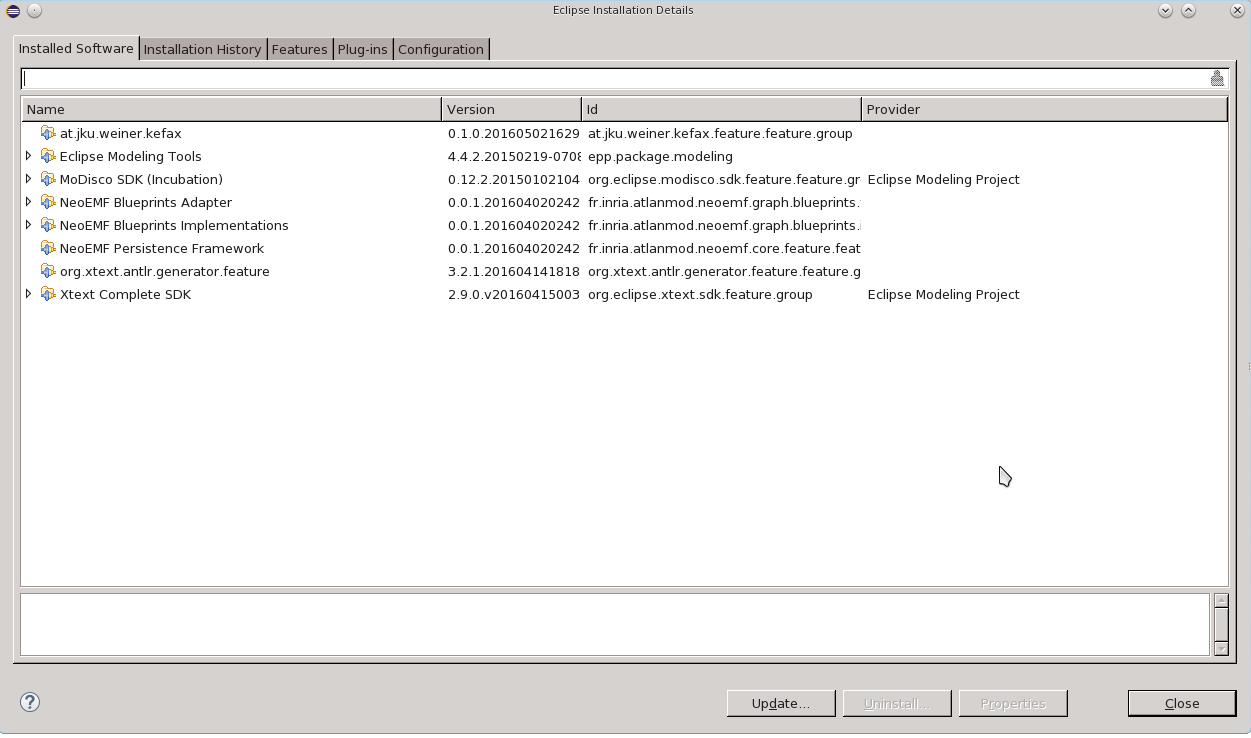
\includegraphics[scale=0.5]{images/install-software}
	\caption{Installation details}
    \label{fig:EclipseInstall}
  \end{figure*}
  \FloatBarrier
  \item Edit the eclipse.ini file. It should contain the following configuration:
  \lstinputlisting[frame=single,extendedchars=true,label=eclipseINI,caption={part of the eclipse.ini},
  breaklines=true,]{code/eclipse.ini}
  \item\label{howToUseRestart} Restart Eclipse
  \item Run by selecting menu items from {\it KeFaX} menu (shown in figure \ref{fig:KefaxMenu}) either
    \begin{itemize}
     \item KeFax $\rightarrow$Run KeFax demonstration A
     \item or KeFax $\rightarrow$Run KeFax demonstration B
    \end{itemize}
\end{enumerate}

 \begin{figure}[ht]
  \centering
  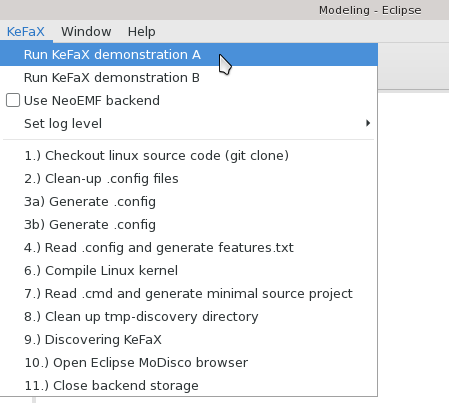
\includegraphics[scale=0.5]{images/kefax-menu-0002}
  \caption{Using KeFaX after installation}
  \label{fig:KefaxMenu}
  \end{figure}
This will now download the Linux source code with git, 
generating a minimal working configuration file, 
execute a kernel compilation to obtain the compile 
options for all source files, generate a {\it features.txt}
file in the destination project {\it kefax-linux-working}, 
copy the minimal required source and header files to the 
{\it kefax-linux-working project} and start discovering the {\it kefax-linux-working project}.
Once pre-processing and parsing is done, 
KeFax will open the {\it MoDisco EMF browser} which shows the 
reverse-engineered Linux kernel C source model. 

Demonstration mode A and demonstration mode B just differ by one feature: 
B has {\it CONFIG\_UNIX98\_PTYS} set to yes will while is not set for A at all. 
This is either done in step {\it 3a) Generate .config} or in step {\it 3b) Generate .config} of the {\it KeFaX} menu. 

The resulting EMF model file(s) can than be found in the folder {\it tmp-discover} of the {\it kefax-linux-working} project. 
\\ \ \\
\begin{figure*}[ht]
  \centering
  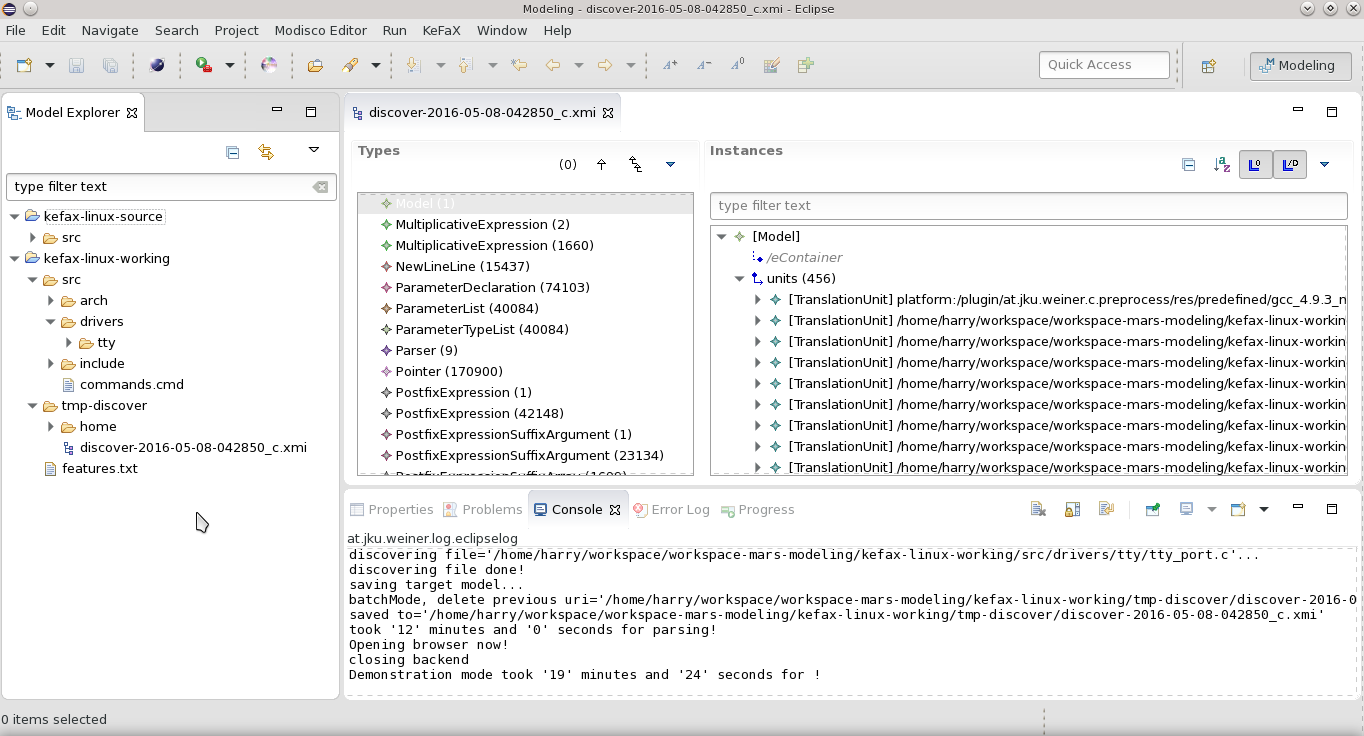
\includegraphics[scale=0.5]{images/discoverer-2015-05-08}
  \caption{Result after running KeFaX}
  \label{fig:discoverer20150508}
\end{figure*}

You might also adjust the log-level or run the individual commands step-wise to see what they are doing in detail.
\\ \ \\
\warning{} Do not run with log-level set to {\it trace}. 
Log-level {\it trace} is only meant to be used for debugging very nasty bugs 
(e.g., preprocessor macro expansion).
It will take almost forever to execute the preprocessor due to printing the detailed log to the console.
Use at your own risk\dots{} You have been warned ;-).

\FloatBarrier

\subsection{How-To develop}
The whole project is distributed under Eclipse Public License - v 1.0 
\cite{EPL_URL} unless otherwise stated.
The source code can be obtained  with git from \url{https://github.com/timeraider4u/kefax}\cite{Kefax2_URL}
\begin{enumerate}
 \item \begin{lstlisting}[language=Bash,breaklines=true,]
        git clone https://github.com/timeraider4u/kefax
       \end{lstlisting}
 \item Execute steps \ref{howToUseDownload} -- \ref{howToUseXtextInstall} from How-To use \ref{sec:howToUse}
 \item Add \url{https://timeraider4u.github.io/kefax/}\cite{Kefax_URL} as an update site, 
 just like in step \ref{howToUseKefaxInstall} of How-To use, but instead of installing {\it kefax} 
 select {\it at.jku.weiner.xtexttest/at.jku.weiner.xtexttest version 0.1.0.201605080110}
 \item Restart Eclipse
 \item Import project into workspace (File $\rightarrow$ Import $\rightarrow$ General $\rightarrow$ 
 Existing projects into workspace) and select the workspace folder inside the local {\it kefax}
 git repository as the root directory. Select all projects and start the import process.
 \item 6. If there are any errors/failures shown after importing you may try to execute 
 Project $\rightarrow$ Clean $\rightarrow$ Clean all projects.
 This will remove temporary Xtext/Xtend files and enforce a global rebuild.
 \item The code structuring will be explained later in this paper. 
 \item KeFaX uses Maven (and Github Travis) for continuous integration:
 A local Maven 3.0 build can be started by navigating to the local kefax git repository root and executing 
 \item \begin{lstlisting}[language=Bash,breaklines=true,]
 mvn clean install
 \end{lstlisting}. This will also execute all JUnit tests.
 \item Feel free to start a pull request or report an issue on the Github page \cite{Kefax2_URL}.
  \begin{itemize}
   \item The {\it master} branch is used for development
   \item The {\it gh-pages} branch is used to store the Eclipse update site. 
  \end{itemize}
 \item Also take a look at the {\it README.md} file 
 and execute git pull from time to time to keep in touch with the latest changes. 
\end{enumerate}

% % !TeX encoding = UTF-8
% !TeX spellcheck = en_US
\section{Linux kernel configuration/build}
\IEEEPARstart{T}he The Linux kernel is developed by programmers from all around the world 
and can be obtained at \url{https://www.kernel.org/}\cite{Kernel_1}.
A mirrored version of the Linux kernel can be found at \url{https://github.com/torvalds/linux}\cite{Kernel_2}.
The kernel is developed, compiled and installed by using Unix-like tools.
The main documentation is provided as plain text files while the kernel itself is programmed 
in the C programming language. Although the kernel itself is developed in C and Assembler,
some of the included helper tools are written in C++, in Bash shell scripts, or even in Python 
(e.g., see {\it tools/perf/python/}) or in Perl (e.g., see {\it tools/perf/perl}).
The Linux kernel also uses its own ecosystem of ``programming languages'' for configuration and 
building of the binary objects which are somehow ``domain-specific languages'', 
which have historically grown over time. 
\begin{figure*}[ht]
  \centering
  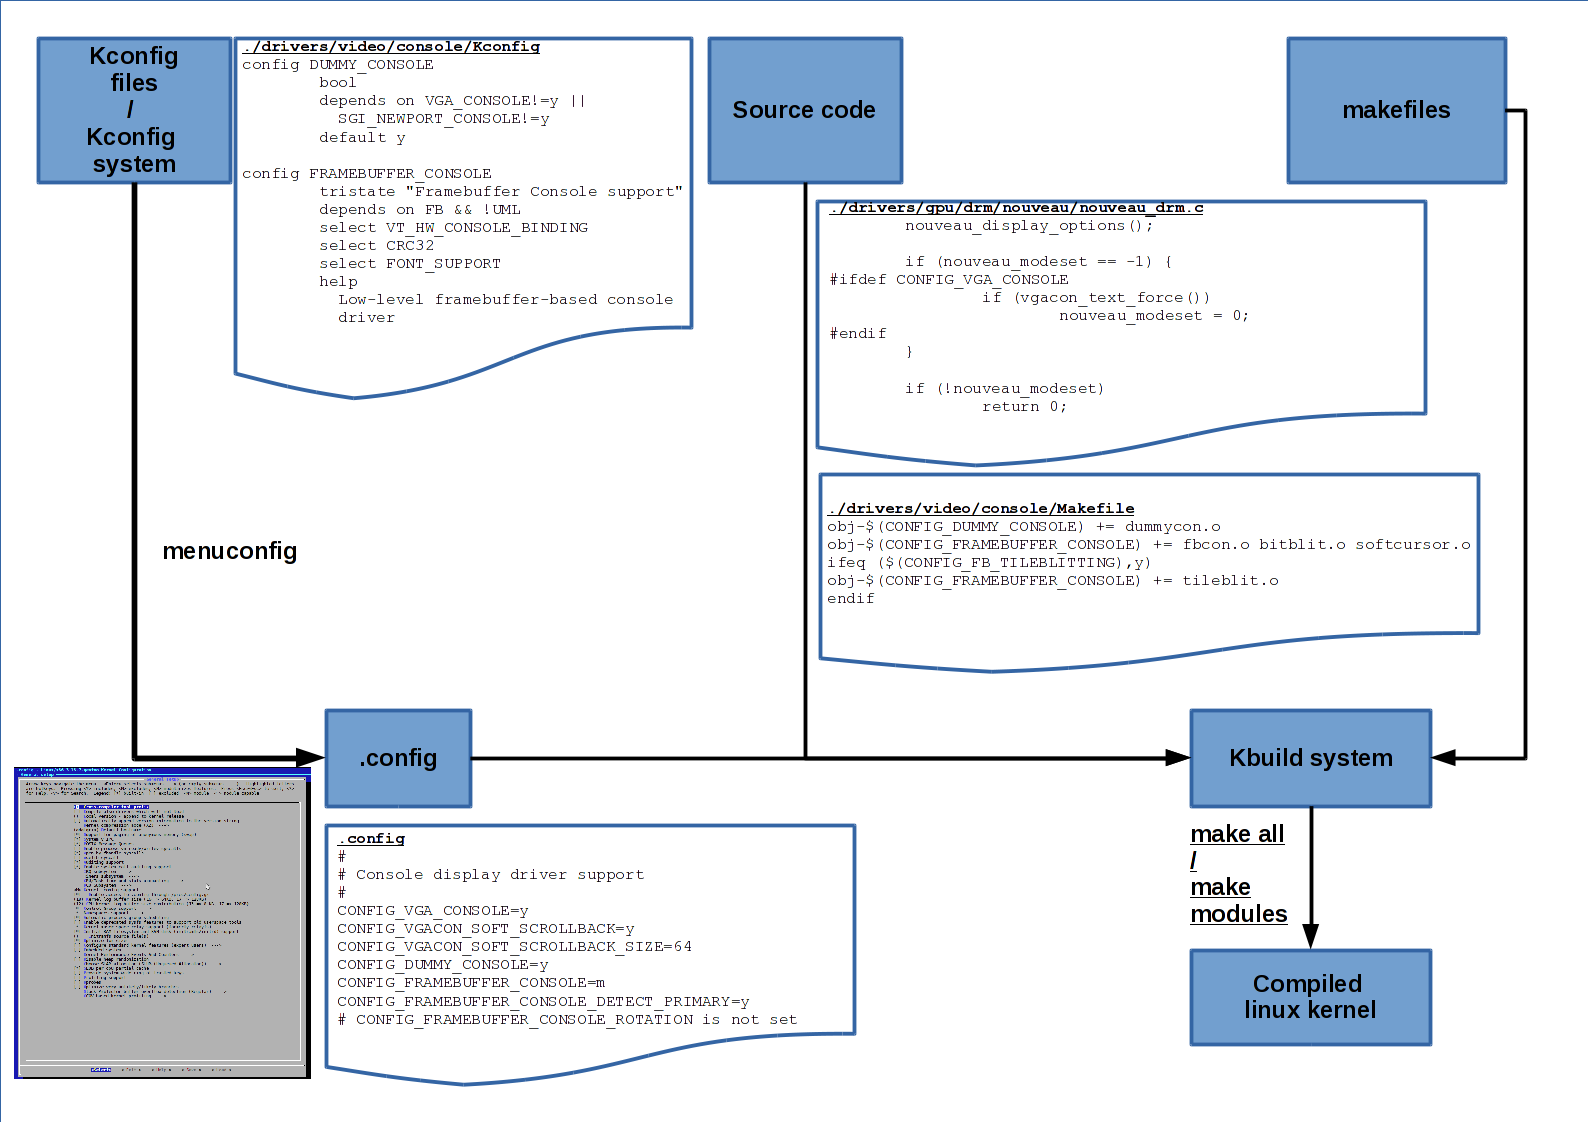
\includegraphics[scale=0.4]{images/overview}
  \caption{Overview over the Linux kernel configuration and build process}
  \label{fig:overview}
\end{figure*}

The picture \ref{fig:overview} shows an overview of the dependencies between the different ``DSLs''.
An overview of the kernel compilation and building can also be found at 
\url{http://www.linuxjournal.com/article/6568}\cite{Kernel_3}

\subsection{.config}

First, the Kconfig system specifies which features depend on each other or can not be combined together. 
Therefore, kconfig serves as some kind of non-formalized feature model.
Here is an example:
\lstinputlisting[frame=single,extendedchars=true,label=Kconfig,caption={./drivers/video/console/Kconfig},
  breaklines=true,]{code/driversVideoConsoleKconfig.txt}

A detailed description of the kconfig system can be found at
\url{https://www.kernel.org/doc/Documentation/kbuild/kconfig-language.txt}\cite{Kernel_4} 
\\ \ \\
The variability model of the Linux kernel is, e.g., described in She et al. 
``The Variability Model of The Linux Kernel''\cite{she2010variability},
in Sincero et al. ``The Linux Kernel Configurator as a Feature Modeling Tool''\cite{sincero2008linux}
and in Tartler et al. ``Dead or alive: finding zombie features in the linux kernel
''\cite{tartler2009dead}.
Although these papers describe older kernel versions their main conclusions are still valid.

\subsection{Generating a .config file}
\begin{figure*}[ht]
  \centering
  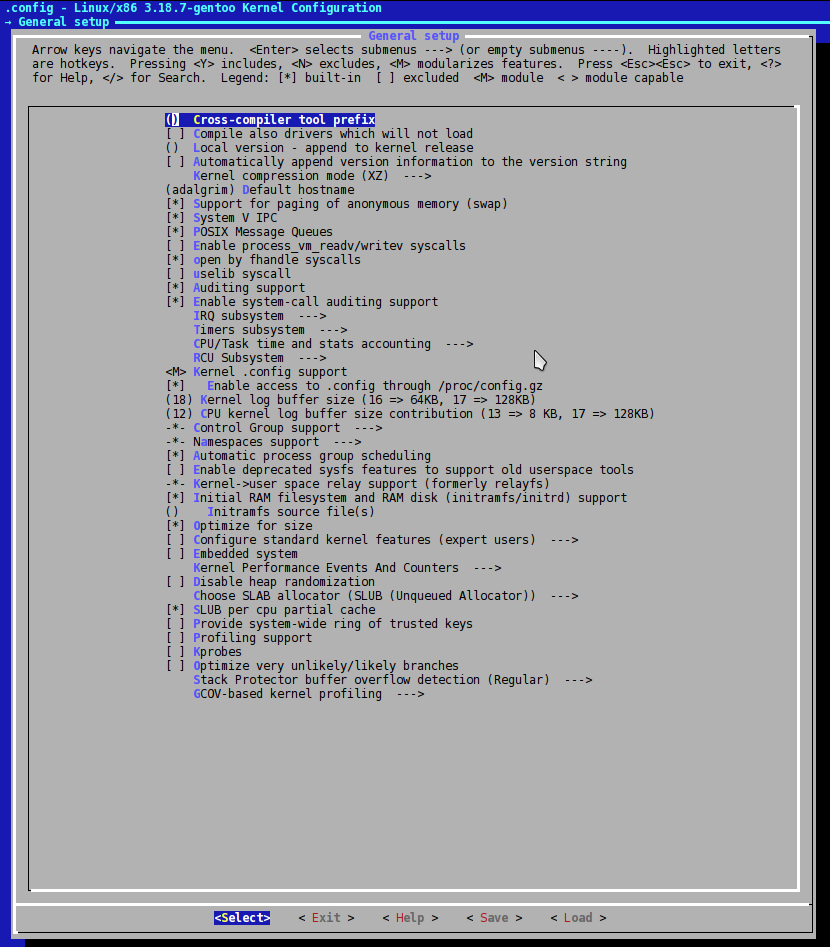
\includegraphics[scale=0.5]{images/menuconfig}
  \caption{Configuring the kernel with menuconfig, e.g., over a ssh connection}
  \label{fig:menuconfig}
\end{figure*}
The users can then use one of the configuration tools which get delivered with the Linux kernel,
e.g. {\it make oldconfig} when you already have a running kernel and you want to only 
update to a new kernel version or 
{\it make menuconfig}, etc.
These applications use the kconfig files as input to determine which additional features 
must be selected or hide options which are not available due to conflicts.
The configuration is then saved into a {\it .config} file at the root directory of the 
Linux kernel source code.

The following text listing is an example for such a generated configuration file:
\lstinputlisting[frame=single,extendedchars=true,label=DotConfig,caption={.config file snippet},
  breaklines=true,]{code/dotConfig.txt}

The following screenshot in figure \ref{fig:menuconfig} 
shows the {\it menuconfig} program, 
a graphical configuration tool which can be used on the terminal:

\subsection{Kbuild system}
Whenever the kernel, its modules or any initramfs should be built the kbuild system is invoked. 
Some valid targets for building are
\begin{itemize}
 \item make all
 \item make kernel
 \item make modules
 \item make vmlinux
 \item make initramfs
\end{itemize}

The makefile in the root directory of the linux source code then invokes the kbuild which 
generates / collects all necessary makefiles and processes them step-wise. 
Most of them just contain plain GNU make instructions but some contain additional bash script magic. 

An example kbuild makefile is the following:
\lstinputlisting[frame=single,extendedchars=true,label=Makefile,caption={Snippet from ./drivers/video/console/Makefile},
  breaklines=true,]{code/MakeFile.txt}
  
The commands in the makefile then instruct the C compiler which source files to compile and 
which command line options to use. The selected features of the {\it .config} file are 
provided as pre-processor macro definitions. But also include directories are enlisted. 

The following source snippet shows how the macro definitions are used in the C source code:
\lstinputlisting[frame=single,extendedchars=true,label=CSourceFile,caption={Snippet from ./drivers/gpu/drm/nouveau/nouveau\_drm.c},
  breaklines=true,]{code/CSourceFile.txt}
The results of the compilation are binary object files which can be installed to 
{\it /boot} and/or {\it /lib/modules/$<$linux-version$>$} with {\it make install}. 

More information about kbuild itself can be found at
\url{https://www.kernel.org/doc/Documentation/kbuild/makefiles.txt}\cite{Kernel_5}
and
\url{http://hemaprathaban.blogspot.co.at/2013/06/makefile-and-kconfig.html}\cite{Kernel_6}

\FloatBarrier

% % !TeX encoding = UTF-8
% !TeX spellcheck = en_US
\section{Required code structure for ECCO}
\IEEEPARstart{E}cco requires a structure similiar to the
file tree shown in figure \ref{fig:overview-2} to be able to parse the product
\\ \ \\
\begin{figure*}[ht]
  \centering
  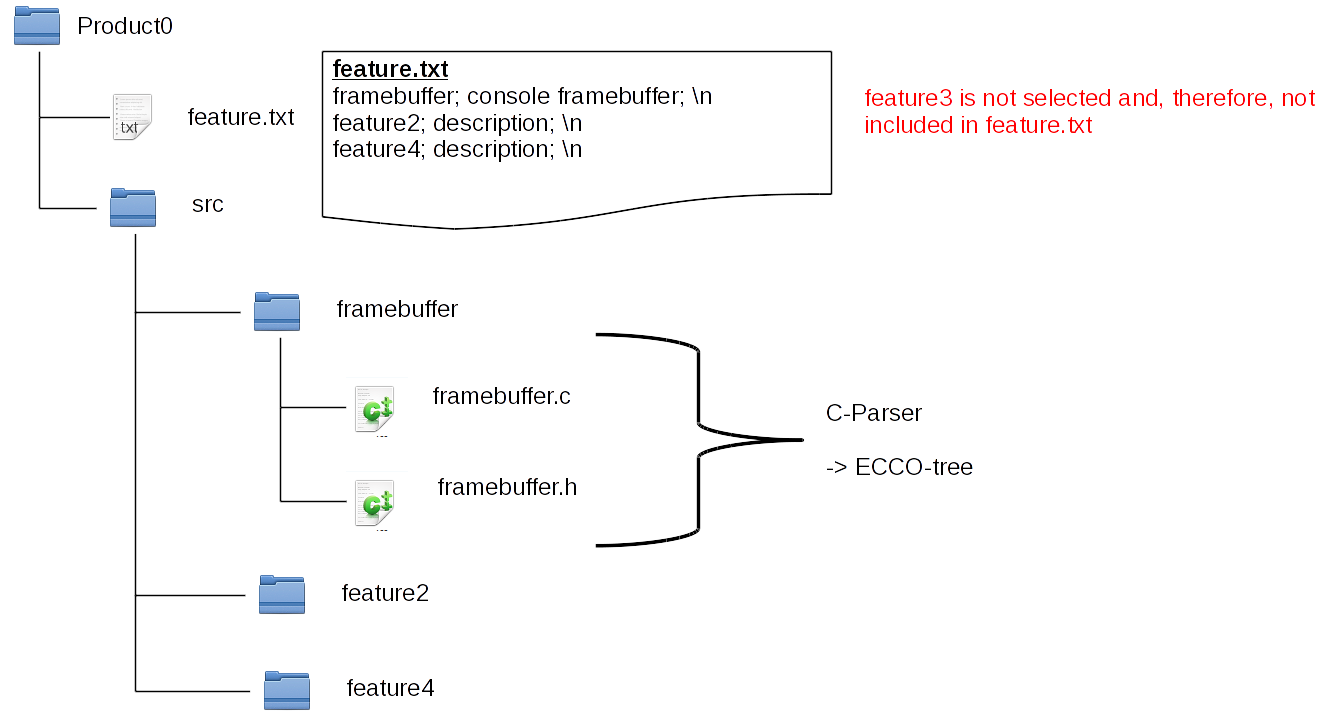
\includegraphics[scale=0.5]{images/overview-2}
  \caption{Overview of required code structure}
  \label{fig:overview-2}
\end{figure*}

The {\it feature.txt} should list all enabled features,
one per line starting with a unique name separated with a semicolon from the feature's description 
and a new-line character at the end.
The file structure should only contain the pruned source code
(so no folders / source files for disabled features). 
The source files should be parsed by some parser and be presented to {\it ECCO} as a tree data structure.

\FloatBarrier

% % !TeX encoding = UTF-8
% !TeX spellcheck = en_US
\section{KeFaX requirements / KeFaX tasks}
\IEEEPARstart{A}s a result of the required input structure of {\it ECCO}, 
the following coarse tasks can be identified for this project:
\begin{enumerate}
 \item Parsing .config file
 \item Obtaining compilation options (which source files are required to be 
 parsed, which include directories are used)
 \item Pre-processing source code and removing un-taken 
 pre-processor conditionals
 \item Parsing source code (.c / .h files)
 \item ``Glue code'' $+$ (Complete data model)
 \item Providing the data structure somehow to {\it ECCO}
\end{enumerate}
\ \\
\ \\
These steps can then be re-defined as:
\begin{enumerate}
 \item\label{reqTaskFeatureCreate} Manually create {\it .config} by selecting features 
 (e.g., in {\it menuconfig})
 \item\label{reqTaskParseDotConfig} Parse {\it .config}
 \item\label{reqTaskFeatureTxtCreate} Create {\it features.txt}
 ({\it .config} $\rightarrow$ {\it features.txt})
 \item\label{reqTaskCompileOptions} Obtain compilation options from kbuild makefiles
 \item\label{reqTaskPruneSource} Prune source code files
 (code files for features that are not selected should be deleted)
 ({\it .config} $+$ makefiles $\rightarrow$ code structure)
 \item\label{reqTaskPreprocess} Run pre-processor on files and do fine-grain
 ({\it \# ifdef} code which is not selected should be thrown away)
 ({\it .config} $\rightarrow$ source code files)
\end{enumerate}


% % !TeX encoding = UTF-8
% !TeX spellcheck = en_US
\section{Implementation}
\IEEEPARstart{T}his chapter will clarify the development history, 
discovered bugs and design decisions taken.

\subsection{Evaluation of existing tools}
Let us first take a look on programs 
which already existed when this project started and 
why they have or have not been used  for KeFaX:

\subsubsection{Using existing compilers / compiler-generators}
C/C++ are very complex programming languages with a lot of disambiguties,
lots of different revisions (e.g. ANSI C, ISO/IEC C99\cite{ISOC99}, C++11) and a 
huge amount of compiler specific extensions
(GNU GCC extensions, etc.). 
The Linux kernel makes use of some of the GNU C extensions.
Therefore, it is not possible to compile the vanilla sources of the Linux kernel with Clang
LLVM yet - the Clang front-end\cite{ClangIntro} would provide a nice abstract syntax tree (AST), 
e.g., as a XML file. For compiler generators like CocoR\cite{COCOR}, 
GNU's implementation of Yacc called Bison\cite{Bison}, etc. there is no unique 
and/or clear EBNF available for C/C++ which would also include most of the GNU C extensions.
A little out-dated grammar  for GNU GCC can be found at \cite{GNUCEBNF}.
GNU gcc itself provides its internal data structures to external programs.
Applications might use this information and provide AST as XML, e.g.
XOgastan\cite{XOgastan} or 
GCC\_XML \cite{gccxml}
The problem with these tools is that they are either not available anymore or are out-dated or buggy.
But even if they would work, the next question is how to build-up the AST, 
which tools and which data structures to use and how much effort would be required to do so \dots

\subsubsection{Reverse Engineering}
Inspired by Schneiden et al. "Model-Based Mining of Source Code Repositories"
\cite{scheidgen2014model} the idea came up that it might be interesting to develop
an {\it Eclipse MoDisco discoverer} \cite{Modisco_1}
\cite{bruneliere2010modisco}
\cite{bruneliere2014modisco}.
{\it Eclipse MoDisco} is a reverse-engineering framework which is built on top of the
{\it Eclipse EMF} (Eclipse Modeling Framework)..
This would solve the question of which data structure / abstract syntax tree
to use for storage.
Discoverers are a set of Eclipse plug-ins that provide an importer/parser for a 
certain programming language.
There exist discoverers for Java, JSP, JSON and many more.
Unfortunately, {\it Eclipse MoDisco discoverers} for C and C++ 
did not exist when starting this project.


% % !TeX encoding = UTF-8
% !TeX spellcheck = en_US
\section{FAQ - Frequently asked questions}
\IEEEPARstart{T}his section lists some frequently asked questions
(or what I suppose to be interesting facts for the public\dots

\begin{center}
\begin{tabular}{|p{5cm}|p{10cm}|}\hline
Question & Answer \\ \hline
Can I use another (probably newer) version of 
{\it org.xtext.antlr.generator} or
{\it Xtext}? 
& No! There have been several changes made to these
software products which are the moment not available
in upstream. There are also some bugs which prevent
me from efficiently getting these changes d'accord
with the master branches, e.g. see bug reports at
\cite{Xtext_bug_1} \cite{Xtext_bug_2} which
themselves required that a bug/feature request
in the {\it EMF genmodel}
generator\cite{EMF_bug_1} needs to be
fixed first.
Anyway, even if I could start a pull request for
the changes made so far, it would be questionable
if they get integrated into the git head at anytime.
\\     \hline
Can I use another (probably newer) version of 
{\it Eclipse MoDisco} or {\it NeoEMF}?
& Yes, you might give them a try. Please
report if newer versions work / do not work for you.
You may use the official update site for 
{\it NeoEMF} because the issues reported in 
\cite{NeoEMF_issue_7}
and \cite{NeoEMF_issue_8} have already been merged
into the master branch and made their way into the 
{\it NeoEMF} official update site.
\\    \hline
%× & ×\\    \hline
%× & ×\\    \hline
%× & × \\   \hline
\end{tabular}
\end{center}


% % !TeX encoding = UTF-8
% !TeX spellcheck = en_US
\section{Lessons learned}
\IEEEPARstart{A} summary of the lessons learned so far \dots

\begin{itemize}
 \item The C programming language has a complex grammar,
 even without pre-processing directives and compiler
 extensions, with lots of disambiguties.
 \item Therefore, there is no {\it Text-To-Model} tool
 availabel yet which supports such a
 complex general programming 
 language like C.
 \item A tool based on {\it ANTLR v4} would be great,
 as {\it ANTLR v3} no longer receives support and
 version 4 is a lot more convinient
 (e.g., semantic predicates no longer needed,
 tree view on default, AST tree walker moved out of
 grammar itself, etc.). Also more grammars
 for version 4 exist and would, therefore, 
 work out-of-the-box.
 \item It would have been nice to have a dedicated
 testing DSL for engineering DSLs. When constructing
 a DSL it is often necessary to check each step of
 the translation process (lexing, parsing and 
 code generation) in detail.
 But the test cases get huge and complex
 when trying to assert 
 that
 lexer tokens, AST tree structures and the output
 files are each correct.
 The DSL used for testing {\it Xtext} projects
 used in this project called {\it XtextTest} has been
 a workaround for this situation, but it is obviously 
 a poor solution to the problem.
 \item Another interesting problem for further research
 would be the co-evolution of abstract and concrete syntax
 (together with automated refactoring of test cases)
 during developing a DSL. E.g., you write your grammar and
 test it on files. Then you have to change the grammar a bit
 to also include some special cases. 
 As a result of the improvements made to the DSL,
 the metamodel has to be changed too and then the code
 generation is not working anymore.
 After fixing the code generation you find out that
 also several dozens or even more of your JUnit tests 
 have to be adapted too to reflect the newest features 
 in the latest version of the DSL.
 This is awkward! Some evolutionary semi-automatical 
 approach would be helpful here, maybe 
 the development of
 several DSLs would
 make sense here: The first DSL for describing the
 concrete syntax could be, e.g., an {\it ANTLR} grammar file.
 The second DSL describes the abstract syntax (the meta-model).
 And then there is a third DSL which actually does the 
 mapping between abstract and concrete syntax. And all of
 them are updated whenever a single line of these DSLs is 
 changed.
\end{itemize}




% An example of a floating figure using the graphicx package.
% Note that \label must occur AFTER (or within) \caption.
% For figures, \caption should occur after the \includegraphics.
% Note that IEEEtran v1.7 and later has special internal code that
% is designed to preserve the operation of \label within \caption
% even when the captionsoff option is in effect. However, because
% of issues like this, it may be the safest practice to put all your
% \label just after \caption rather than within \caption{}.
%
% Reminder: the "draftcls" or "draftclsnofoot", not "draft", class
% option should be used if it is desired that the figures are to be
% displayed while in draft mode.
%
%\begin{figure}[!t]
%\centering
%\includegraphics[width=2.5in]{myfigure}
% where an .eps filename suffix will be assumed under latex, 
% and a .pdf suffix will be assumed for pdflatex; or what has been declared
% via \DeclareGraphicsExtensions.
%\caption{Simulation Results}
%\label{fig_sim}
%\end{figure}

% Note that IEEE typically puts floats only at the top, even when this
% results in a large percentage of a column being occupied by floats.


% An example of a double column floating figure using two subfigures.
% (The subfig.sty package must be loaded for this to work.)
% The subfigure \label commands are set within each subfloat command, the
% \label for the overall figure must come after \caption.
% \hfil must be used as a separator to get equal spacing.
% The subfigure.sty package works much the same way, except \subfigure is
% used instead of \subfloat.
%
%\begin{figure*}[!t]
%\centerline{\subfloat[Case I]\includegraphics[width=2.5in]{subfigcase1}%
%\label{fig_first_case}}
%\hfil
%\subfloat[Case II]{\includegraphics[width=2.5in]{subfigcase2}%
%\label{fig_second_case}}}
%\caption{Simulation results}
%\label{fig_sim}
%\end{figure*}
%
% Note that often IEEE papers with subfigures do not employ subfigure
% captions (using the optional argument to \subfloat), but instead will
% reference/describe all of them (a), (b), etc., within the main caption.


% An example of a floating table. Note that, for IEEE style tables, the 
% \caption command should come BEFORE the table. Table text will default to
% \footnotesize as IEEE normally uses this smaller font for tables.
% The \label must come after \caption as always.
%
%\begin{table}[!t]
%% increase table row spacing, adjust to taste
%\renewcommand{\arraystretch}{1.3}
% if using array.sty, it might be a good idea to tweak the value of
% \extrarowheight as needed to properly center the text within the cells
%\caption{An Example of a Table}
%\label{table_example}
%\centering
%% Some packages, such as MDW tools, offer better commands for making tables
%% than the plain LaTeX2e tabular which is used here.
%\begin{tabular}{|c||c|}
%\hline
%One & Two\\
%\hline
%Three & Four\\
%\hline
%\end{tabular}
%\end{table}


% Note that IEEE does not put floats in the very first column - or typically
% anywhere on the first page for that matter. Also, in-text middle ("here")
% positioning is not used. Most IEEE journals/conferences use top floats
% exclusively. Note that, LaTeX2e, unlike IEEE journals/conferences, places
% footnotes above bottom floats. This can be corrected via the \fnbelowfloat
% command of the stfloats package.


% trigger a \newpage just before the given reference
% number - used to balance the columns on the last page
% adjust value as needed - may need to be readjusted if
% the document is modified later
%\IEEEtriggeratref{8}
% The "triggered" command can be changed if desired:
%\IEEEtriggercmd{\enlargethispage{-5in}}

% references section

% can use a bibliography generated by BibTeX as a .bbl file
% BibTeX documentation can be easily obtained at:
% http://www.ctan.org/tex-archive/biblio/bibtex/contrib/doc/
% The IEEEtran BibTeX style support page is at:
% http://www.michaelshell.org/tex/ieeetran/bibtex/
\bibliographystyle{IEEEtran}
% argument is your BibTeX string definitions and bibliography database(s)
\bibliography{kefax}
%
% <OR> manually copy in the resultant .bbl file
% set second argument of \begin to the number of references
% (used to reserve space for the reference number labels box)
%\begin{thebibliography}{1}

%\bibitem{IEEEhowto:kopka}
%H.~Kopka and P.~W. Daly, \emph{A Guide to \LaTeX}, 3rd~ed.\hskip 1em plus
%  0.5em minus 0.4em\relax Harlow, England: Addison-Wesley, 1999.

%\end{thebibliography}




% that's all folks
\end{document}


